\subsection{Definition}
\begin{frame}
  \frametitle{Definition}
  \begin{block}{Zweck}
Das Visitor Pattern ermöglicht es, neue Operationen auf den Elementen einer Struktur zu definieren, ohne die Elemente selbst anzupassen.
  \end{block}
\end{frame}

\subsection{Klassendiagramm - Visitor Pattern}
\begin{frame}
	\frametitle{Klassendiagramm}		
	\begin{itemize}
		\item Anzahl unterschiedlicher Elemente der Objektstruktur fest
	\end{itemize}	
  	\begin{figure}
		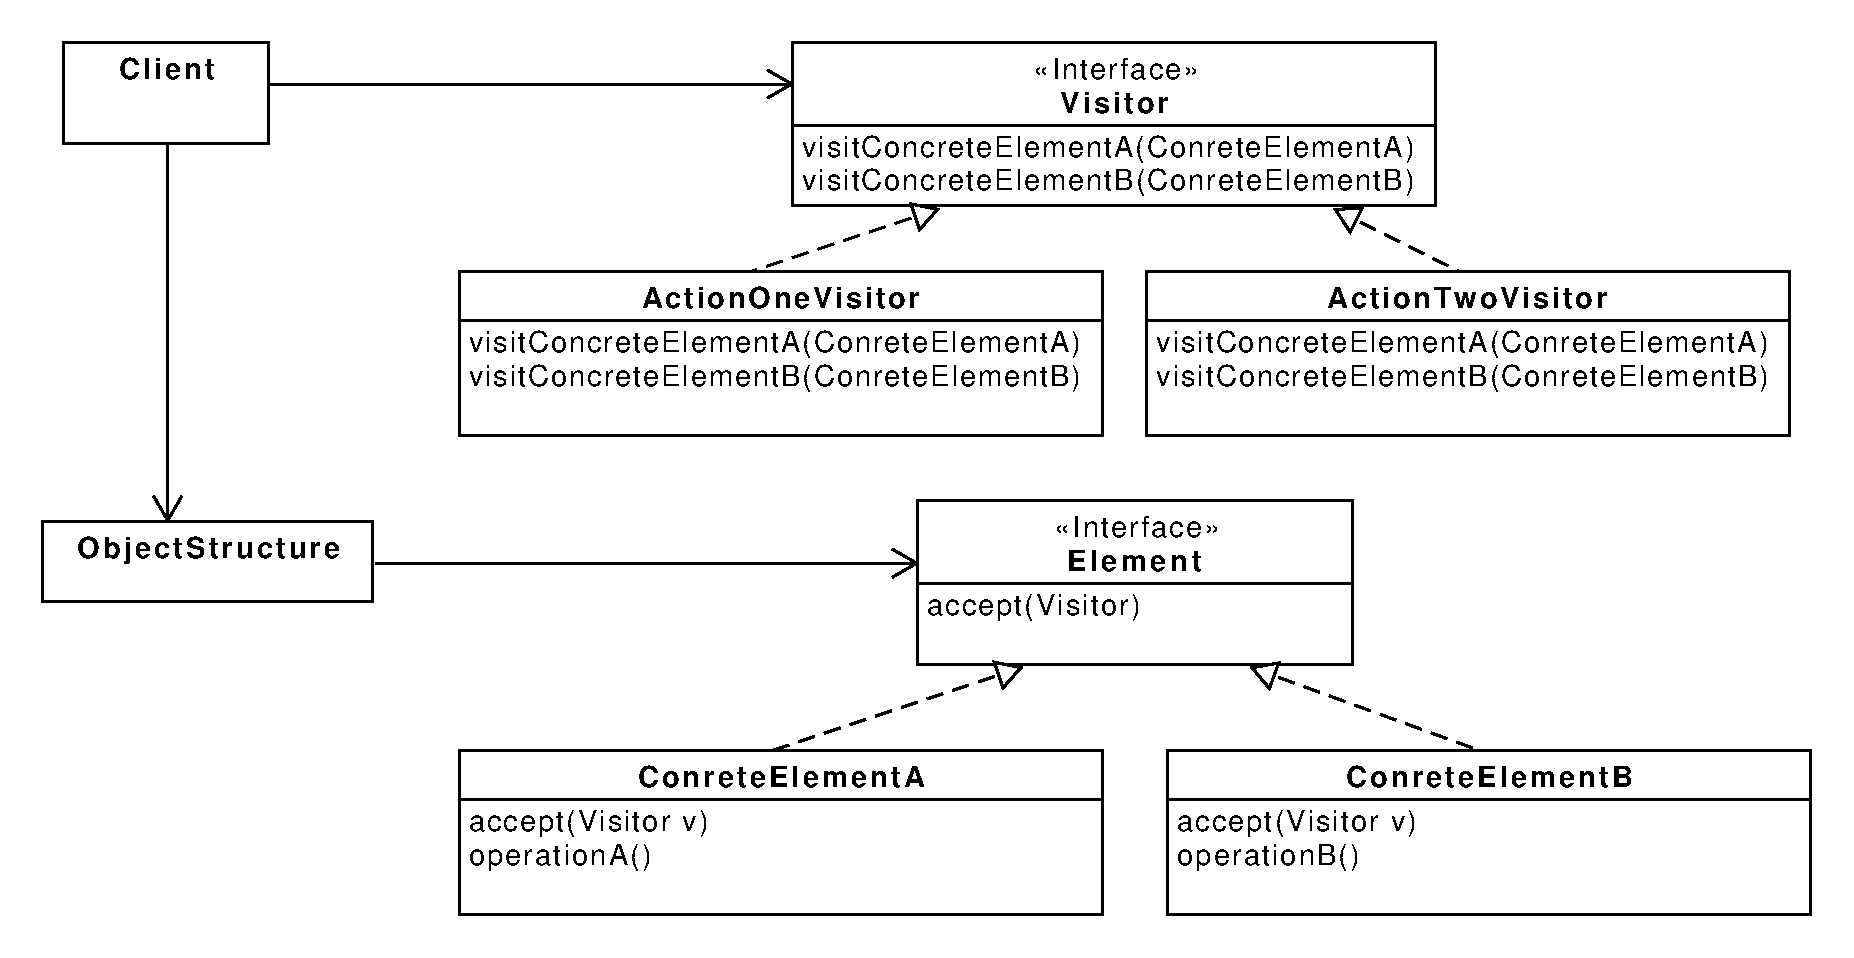
\includegraphics[scale=.3]{paper/visitor/visitor}
	\end{figure}
\end{frame}

\subsection{Beispiel - Kitchen}
\begin{frame}
	\frametitle{Beispiel}
	\begin{itemize}
		\item Die verschiedenen Sorten die wir bearbeiten möchten, bleiben konstant
		\item Wie wir diese bearbeiten ist noch unklar.
	\end{itemize}	
	
  	\begin{figure}
		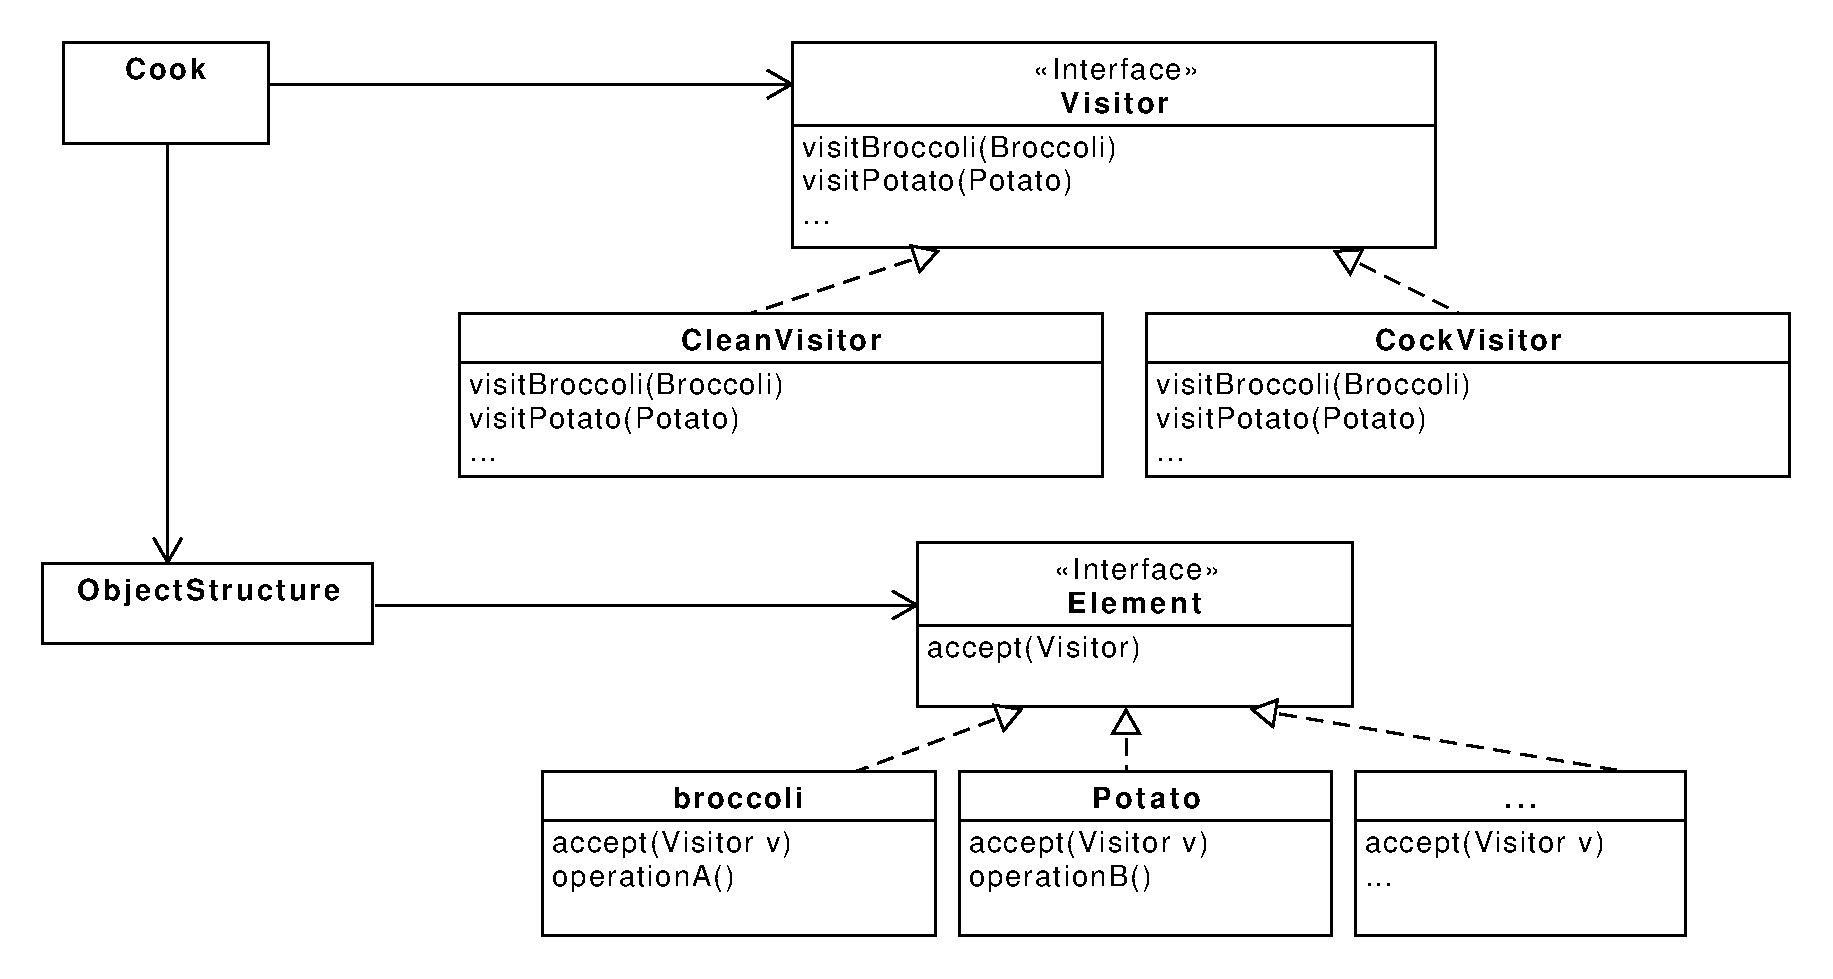
\includegraphics[scale=.3]{paper/visitor/kitchen}
	\end{figure}
\end{frame}



\begin{frame}
	\frametitle{Beispiel}
  	\begin{figure}
		\javacode{resources/visitor_element_interface.java} 
		\javacode{resources/visitor_visitor_interface.java}
	\end{figure}
\end{frame}

\begin{frame}
	\frametitle{Beispiel}
  	\begin{figure}
		\javacode{resources/visitor_potato.java} 
		\javacode{resources/visitor_cleanvisitor.java}
	\end{figure}
\end{frame}

\begin{frame}
	\frametitle{Beispiel}
  	\begin{figure}
		\javacode{resources/visitor_main.java} 
	\end{figure}
\end{frame}

\begin{frame}
	\frametitle{Beispiel}		
	\begin{itemize}
		\item Der Client erstellt die Instanzen cleanVisitor, potato und broccoli
		\item Übergibt Elemente über Accept-Methode(potato und broccoli) den Visitor
		\item Elemente rufen die jeweilige Visit-Methode auf und übergeben sich selbst zur Bearbeitung
	\end{itemize}	
  	\begin{figure}
		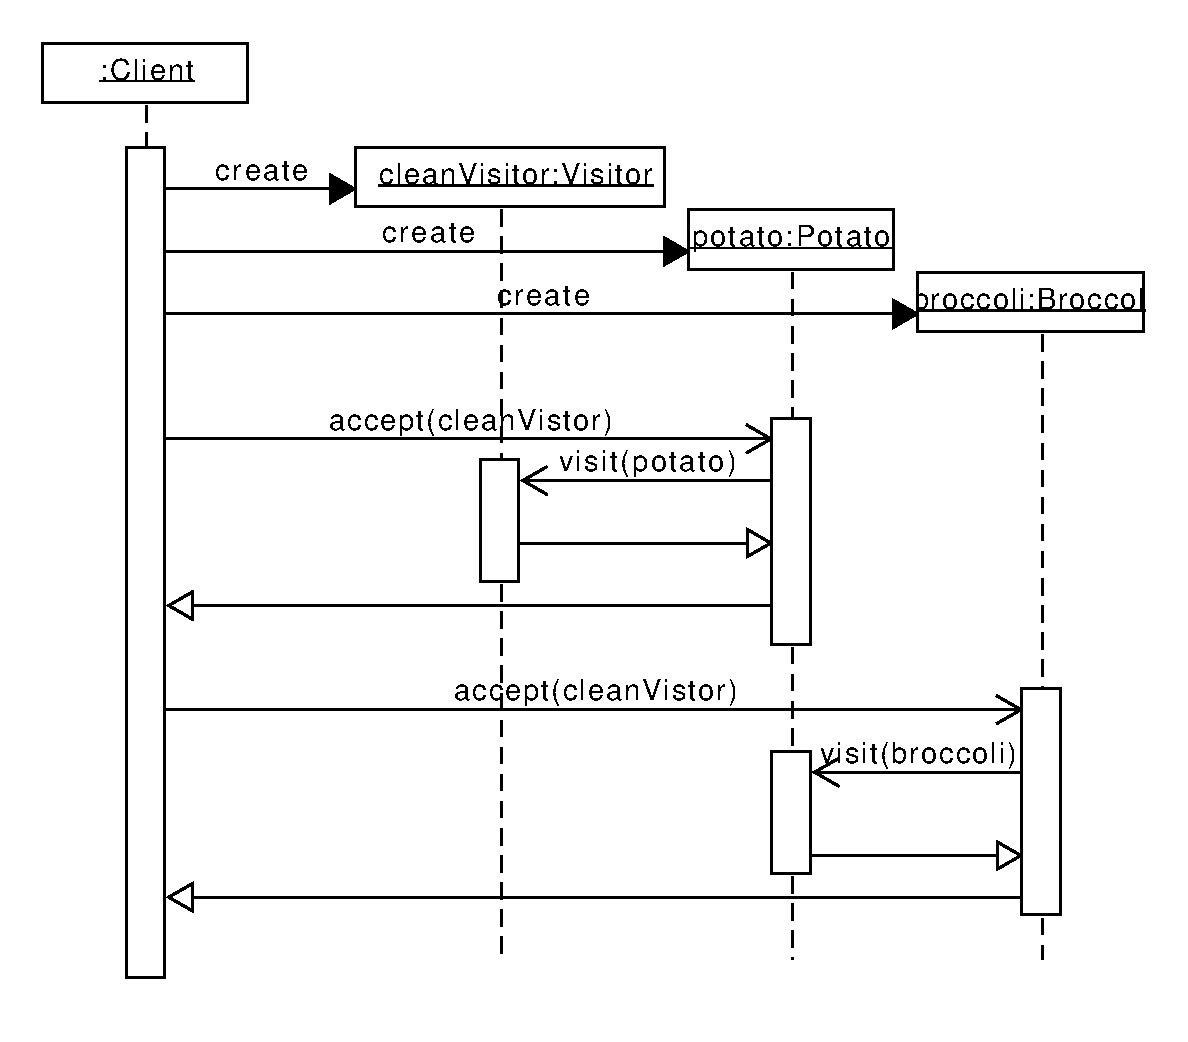
\includegraphics[scale=.29]{paper/visitor/visitor_sequenz}
		                                        
	\end{figure}
\end{frame}




\begin{frame}
	\frametitle{Implementierungsmöglichkeiten}
  \begin{block}{Wer ist für die Traversierung der Objektstruktur verantwortlich}
  	\begin{itemize}
  		\item Die Objektstuktur
  		\item Ein Iterator
  		\item Das Visitor-Objekt
  	\end{itemize}
  \end{block}
\end{frame}


\begin{frame}
	\frametitle{Implementierungsmöglichkeiten}
  \begin{block}{Objektstruktur}
  	\begin{itemize}
  		\item Objektstruktur kümmert sich um die Traversierung 
  		\item Visitor muss der Objektstruktur übergeben werden
  		\item Realisierbar durch z.B Composite-Pattern
  	\end{itemize}
  \end{block}
  \javacode{resources/visitor_composide_example.java} 
\end{frame}

\begin{frame}
	\frametitle{Implementierungsmöglichkeiten}
  \begin{block}{Iterator}
  	\begin{itemize}
  		\item Abstraktion zum Zugriff auf Elemente einer Objektstruktur, ohne die  Objektstruktur zu kennen.
  		\item Visitor-Objekt wird dem Iterator übergeben
  		\item Beim Zugriff eines Elements die accept-Methode aufrufen

  	\end{itemize}
  \end{block}
	\begin{block}{Im Visitor-Objekt}
  	\begin{itemize}
  		\item Objektstruktur wird den konkreten Visitors übergeben
  		\item Visitor übernimmt jetzt die Traversierung
  		\item Nachteil: Traversierung in jedem Visitor
  		\item Vorteil: Möglichkeit, die Objektstruktur unterschiedlich zu durchlaufen
  	\end{itemize}
  \end{block}
\end{frame}


\begin{frame}
	\frametitle{Implementierungsmöglichkeiten}

  \javacode{resources/visitor_trav_visitor_object.java} 
\end{frame}

\subsection{Fazit}
\begin{frame}
	\frametitle{Fazit}
	\begin{columns} 
    	\column[t]{.50\textwidth} 
    		\begin{exampleblock}{Vorteile}
    			\begin{itemize}
    				\item Leicht neue Operationen auf eine Objektstruktur zu implementieren
    				\item Selektives bearbeiten einzelner Elemente einer Objektstruktur
    			\end{itemize}
    		\end{exampleblock}
    	\column[t]{.50\textwidth} 
    		\begin{alertblock}{Nachteile}
    			\begin{itemize}
    				\item Enge Kopplung des Visitor mit den Elementen einer Objektstruktur
    				\item Elemente müssen über öffentliche Methoden und Attribute den Zugriff bereitstellen
    			\end{itemize}
    		\end{alertblock}
  	\end{columns}   	  		
\end{frame}